\subsection{\textsc{K-Dist} algorithm}

This section presents the \textsc{K-Dist} algorithm used in \texttt{klust}.

\textsc{K-Dist} uses a window of length equal to the shortest of the two
sequences being compared. The distance between the substrings in the initial,
leftmost position of the window is calculated using a variant (described below)
of the basic \textsc{d2} algorithm (algorithm \ref{alg:d2_basic}) described in
section \ref{sec:kmer_distance}. The window then iterates over the longer
sequence and calculates the new distance between the substring of the longer
sequence and the shorter sequence.  This calculation is done using a kind of
forward differences method for reducing the calculations to a few fixed
operations for calculating the distance in the next window from the distance in
the current window. This concept is described in~\cite{hazelhurst}.

\textsc{K-Dist} uses the \emph{Manhattan distance} instead of the Euclidean
distance used in the \textsc{d2} algorithm for calculating the distance between
the two $k$-mer frequency vectors. The Manhattan distance is similar to the
Euclidean distance but with squaring replaced with absolute value and the
square root omitted, i.e.  for $u, v \in \mathbb{Z}^n$,

\begin{equation}
  d_{Manhattan} \eqdef \sum_{i=1}^{n} |u_i - v_i| \;.
\end{equation}

This distance metric was chosen for simplicity, to make the calculation of
distance in subsequent window positions easier, which also improves
performance, and since there is evidence in the literature that the Manhattan
distance generally is preferable to Euclidean distance for high dimensional
distance calculation~\cite{aggarwal}.  % TODO: more about Euclidean being bad

To calculate the distance in the next window position from the distance in the
current window, i.e. advancing the window through the longer of the two
sequences by one character, it is decided which $k$-mers exit and enter the
window, respectively, and then by looking at whether the existing $k$-mer count
in the frequency vector is negative or positive, it can be decided whether the
distance increases or decreased by 2 or whether it stays the same.
Subsequently, the frequency vector is updated to reflect the change in the new
window. Figure \ref{fig:d2_forward_differences} illustrates the idea of a
window and $k$-mers exiting and entering the window:

\begin{figure}[H]
\centering
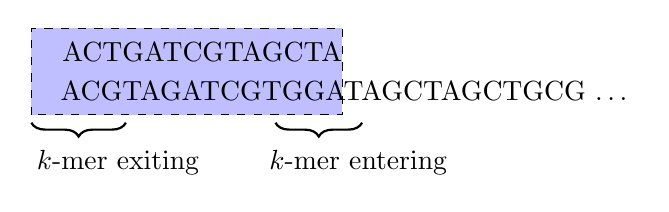
\begin{tikzpicture}
  \draw [fill=blue!25,dashed] (0,0.7) rectangle (3.95,1.8);
  \node at (4.0,1.5) {ACTGATCGTAGCTA\phantom{TAGCTAGCTGCG \dots}};
  \node at (4.0,1.0) {ACGTAGATCGTGGATAGCTAGCTGCG \dots};
  \draw [thick,decorate,decoration={brace,amplitude=5pt,mirror}]
    (0.0,0.6) -- (1.2,0.6) node[midway,xshift=0.5cm,yshift=-0.5cm]
    {$k$-mer exiting};
  \draw [thick,decorate,decoration={brace,amplitude=5pt,mirror}]
    (3.1,0.6) -- (4.2,0.6) node[midway,xshift=0.5cm,yshift=-0.5cm]
    {$k$-mer entering};
\end{tikzpicture}
\caption{Illustration of $k$-mers entering and exiting a window.}
\label{fig:d2_forward_differences}
\end{figure}

A distance measure, i.e. not a relative similarity measure, can be difficult to
use for determining sequence similarity since the distance metric is very
dependent on the length of the shortest sequence (the length of the window).

For this reason, the ratio between the Manhattan distance and the maximum
possible distance in the window is used to normalize the distance to a value in
the interval $[0,1]$. Let $w$ denote the size of the window. The corresponding
similarity measure for the distance Manhattan distance in the window is given
by the following:

\begin{equation}
  1 - \frac{d_{Manhattan}(s,t)}{2(w - k + 1)} \label{eq:Manhattan_similarity}
\end{equation}

An alternative notion of similarity, which was the inspiration for the above
similarity measure, is the \emph{Jaccard index}~\cite{jaccard1912}, which is
defined as the size of the intersection of two sets divided by the size of the
union of the sets.  However, the Jaccard index does not take the multiplicity
of the elements into account and therefore it might give a lower sensitivity
than the similarity measure in (\ref{eq:Manhattan_similarity}).

The \textsc{K-Dist} algorithm (algorithm \ref{alg:K-Dist}) has been implemented
and is used as the distance metric in the \texttt{klust} program.

\begin{algorithm}
  \caption{\textsc{K-Dist} algorithm}
  \label{alg:K-Dist}
  \begin{algorithmic}[1]
    \Require{$s$ and $t$ are DNA or RNA sequence, $k \in \mathbb{Z}^+$}
    \Statex
    \Function{K-Dist}{$s, t, k$}
      \State set $s$ to the shorter sequence and $t$ to the longer sequence
      \State initialize array \texttt{kmers} of size $4^k$
      \State $cur\_dist \gets 0$
      \For{$i \gets 0$ to $length(s) - k$}
        %\State \Call{\textsc{Update-Distance}}{($t$.substring($i$, $k$),
        %                $s$.substring($i$, $k$), dist)}
        \State \texttt{kmers}[$s$.substring($i$, $k$)]\texttt{++}
        \Comment{\parbox[t]{.3\linewidth}{$k$-mer counting}}
        \State \texttt{kmers}[$t$.substring($i$, $k$)]\texttt{-{}-}
      \EndFor
      \ForAll{$c \in$ \texttt{kmers}}
        \State $cur\_dist \gets cur\_dist + |c|$
          \Comment{\parbox[t]{.3\linewidth}{Manhattan distance}}
      \EndFor
      \State $min\_dist \gets cur\_dist$
      \For{$i \gets 0$ to $length(t) - length(s)$}
          \Comment{\parbox[t]{.3\linewidth}{No. of windows}}
        \State \texttt{kmers}[$t$.substring($i$, $k$)]\texttt{-{}-}
        \State \texttt{kmers}[$t$.substring($length(s)-k+i+1$, $k$)]\texttt{++}
        \State update $cur\_dist$ to current Manhattan distance
        \State $min\_dist \gets min(min\_dist, cur\_dist)$
      \EndFor
          \State $total \gets 2(length(s)-k+1)$
            \Comment{\parbox[t]{.3\linewidth}{Maximal distance}}
      \State \Return{$(total-min\_dist) / total$}
    \EndFunction
    \Statex
    \Function{Update-Distance}{$\mathtt{arr}, kmer\_exit, kmer\_enter, dist$}
      \If{$\mathtt{arr}[kmer\_exit] > 0$}
        \State $dist \gets dist - 1$
      \Else
        \State $dist \gets dist + 1$
      \EndIf
      \If{$\mathtt{arr}[kmer\_enter] < 0$}
        \State $dist \gets dist - 1$
      \Else
        \State $dist \gets dist + 1$
      \EndIf
    \EndFunction
  \end{algorithmic}
\end{algorithm}


\subsubsection{Time complexity analysis}

The \textsc{K-Dist} algorithm first iterates over the first $|s|-k$ characters,
where $|s|$ denotes the length of the shorter of the two sequences. Each
iteration contains only constant time operations. So far, a running time of
$\Theta(\abs{s}-k)$.

Secondly, the algorithm iterates over the \texttt{kmers} array, which is of
size $4^k$, and performs a single addition for each position.

% TODO: fix algorithm
